% Drift-Sense mid-semester report.
%
% Build (from this directory):
%   tectonic main.tex                      # self-contained, fetches packages
%   or: latexmk -xelatex main.tex          # with a TeX Live / MacTeX install
%
% Figures are read from ../../figures/, so build from reports/midsem/.
% Section files live in sections/; each names the scripts and CSVs its
% numbers come from.
\documentclass[11pt,a4paper]{article}

\usepackage[margin=2.5cm]{geometry}
\usepackage{amsmath,amssymb}
\usepackage{graphicx}
\usepackage{microtype}
\usepackage[section]{placeins}  % keep each figure/table inside its own section
\usepackage[hidelinks]{hyperref}

% File paths and sequence names (\texttt{...}, MH\_01\_easy) cannot be
% hyphenated; let TeX stretch those lines instead of overrunning the margin.
\setlength{\emergencystretch}{3em}

\title{Drift-Sense: Predicting IMU Dead-Reckoning Drift\\from Window-Level Motion Features}
\author{Yatin \and Harsith Priyan Sivanandham \and Pranavi Mathur \and GuruManoharGuptaBaratam}
\date{Mid-semester report}

\begin{document}
\maketitle

% Dataset & EDA section (Part B)
% Include from reports/midsem/main.tex.

\section{Dataset and Exploratory Analysis}
\label{sec:dataset-eda}

\subsection{EuRoC MAV}
Phase~1 uses two Machine Hall sequences from the EuRoC MAV dataset
\cite{burri2016euroc}: MH\_01\_easy and MH\_02\_easy. Each flight is a
few minutes of a real hexacopter with a stereo camera and an ADIS16448
IMU. We use only \texttt{imu0/data.csv} (gyroscope in rad/s,
accelerometer specific force in m/s$^2$, nominally 200\,Hz) and
\texttt{state\_groundtruth\_estimate0/\allowbreak data.csv} (position, Hamilton
quaternion, velocity, and IMU biases). Camera images are reserved for
Phase~2. MH\_03\_medium is not used in this phase.

\subsection{Data quality}
Table~\ref{tab:quality} summarises the two streams after loading.
There are no missing values. Both IMU and the provided ground-truth
estimate are sampled at 200\,Hz with a 5\,ms median step and negligible
jitter. Nearest-timestamp alignment drops 1.17\% and 1.32\% of IMU rows
(MH\_01, MH\_02), almost entirely at sequence edges where ground-truth
coverage starts later than the IMU. We treat those drops as coverage
gaps, not sensor faults.

\begin{table}[htbp]
\centering
\caption{Sequence-level quality checks.}
\label{tab:quality}
\begin{tabular}{lrrrrr}
\hline
Sequence & IMU rows & Duration (s) & Rate (Hz) & Missing & Align drop \\
\hline
MH\_01\_easy & 36820 & 184.1 & 200 & 0 & 1.17\% \\
MH\_02\_easy & 30400 & 152.0 & 200 & 0 & 1.32\% \\
\hline
\end{tabular}
\end{table}

Raw gyro over the first 10\,s of MH\_01 is small-amplitude chatter
($\sim$0.2\,rad/s), i.e.\ noise plus slow attitude change rather than
aggressive spins. Accelerometer magnitude stays near $g$; the vehicle is
pitched, so gravity appears on $a_x$ and $a_z$ together, not on $a_z$
alone.

\subsection{The two easy flights}
The flights occupy a similar machine-hall volume. Mean ground-truth
speed is 0.44\,m/s on MH\_01 and 0.49\,m/s on MH\_02 (peaks about
2.0\,m/s and 1.2\,m/s). Path length is $\sim$81\,m and $\sim$74\,m.
Mean gyro magnitude is $\sim$0.21\,rad/s on both. They are close enough
that leave-one-sequence-out is a fair, if small, generalisation test,
and different enough (duration, path) that holding one out is still
meaningful.

\subsection{Drift label}
The headline target is the 2\,s raw-IMU position error $y=\texttt{err\_mag\_m}$.
Across 720 and 592 overlapping windows the means are 1.215 and 1.203\,m
with standard deviations 0.058 and 0.079\,m. The histograms are tight and
left-skewed (skew $-1.7$, $-2.1$; max 1.34\,m). We therefore
\textbf{do not} log-transform the primary target.

The same windows after subtracting the dataset's ground-truth IMU biases
(\texttt{err\_mag\_m\_bc}) have means 0.063 and 0.054\,m. This
supports the claim that 2\,s raw drift is bias-dominated; the
bias-corrected series is an oracle comparison, not the leaderboard
target. Signed axis errors $({\Delta}x,{\Delta}y,{\Delta}z)$ vary more
than the Euclidean magnitude, so Phase~1 models should also be trained
on the 3-axis target.

Mean error versus window length (0.25--2.0\,s) grows superlinearly for
the raw integrator ($\sim$6\,mm at 0.25\,s to $\sim$1.2\,m at 2\,s) and
remains much smaller after bias correction. The primary window was
changed from 1.0\,s to 2.0\,s (0.25\,s stride) because the longer label is
far more predictable (Section~\ref{sec:window-length}).

\subsection{Train/test protocol}
Windows overlap by 87.5\%. A random split of rows would place nearly
identical IMU slices in both train and test and inflate $R^2$. With two
sequences we still use leave-one-sequence-out, recorded in
\texttt{data/processed/splits.json}: train on MH\_02 and test on MH\_01,
then swap. The leakage test \texttt{tests/test\_no\_leakage.py} asserts
that no sequence appears on both sides of any fold. The primary target
in that file is \texttt{err\_mag\_m}.


\section{Method}
\label{sec:method}
% Method section — Label Construction subsection (Part A)
% Paste this into reports/midsem/sections/method.tex, alongside
% Part C's feature-engineering subsection.
%
% Numbers marked [FILL] should be replaced with your actual run's output
% once make_windows.py has been run and its printed summary recorded.

\subsection{Drift Label Construction}
\label{sec:label-construction}

The EuRoC dataset does not provide a pre-computed odometry-drift signal;
it supplies raw IMU measurements and precise ground-truth pose from a
motion-capture system. We construct the regression target — the position
error that a Visual-Inertial Odometry system would accumulate over a
short time window — directly from these two streams.

\subsubsection{Temporal Alignment}
IMU measurements (200\,Hz) and ground-truth pose estimates are recorded
asynchronously. For every IMU sample we attach the temporally nearest
ground-truth sample, discarding IMU samples whose nearest match exceeds
a 20\,ms tolerance. Across the two sequences used in Phase 1
(MH\_01\_easy and MH\_02\_easy), this discarded between
1.2\% and 1.3\% of IMU samples, concentrated at sequence boundaries
where ground-truth coverage is sparser than IMU coverage.

\subsubsection{Windowing}
The aligned stream is divided into overlapping windows of
$T_w = 2.0\,\mathrm{s}$ (400 IMU samples at 200\,Hz), with a stride of
$T_s = 0.25\,\mathrm{s}$ between consecutive window starts. This yielded
720 and 592 windows for MH\_01\_easy and MH\_02\_easy respectively.
An earlier version used $T_w = 1\,\mathrm{s}$;
Section~\ref{sec:window-length} shows why the longer window was adopted.

\subsubsection{IMU Strapdown Integration}
For each window, we compute a model-free position estimate by
integrating the raw IMU measurements forward using standard strapdown
inertial mechanization. Starting from the true position $p_0$, velocity
$v_0$, and orientation quaternion $q_0$ at the window's first timestamp
(taken directly from ground truth), we integrate at each IMU sample
$i$ with timestep $\Delta t_i$:
\begin{align}
  a_{\text{world},i} &= R(q_i)\, a_{\text{body},i} + g \\
  v_{i+1} &= v_i + a_{\text{world},i}\, \Delta t_i \\
  p_{i+1} &= p_i + v_i \Delta t_i + \tfrac{1}{2} a_{\text{world},i} \Delta t_i^2 \\
  q_{i+1} &= q_i \otimes \Delta q(\omega_i, \Delta t_i)
\end{align}
where $R(q_i)$ is the rotation matrix corresponding to the current
orientation estimate, $g$ is the world-frame gravity vector, and
$\Delta q(\omega_i, \Delta t_i)$ is the incremental rotation from the
gyroscope reading $\omega_i$.

Two sign/frame conventions — the sign of $g$ and whether $R(q_i)$ maps
body-to-world or world-to-body — are not fixed by the dataset
documentation alone and were determined empirically: we evaluated all
four combinations on a short (0.25\,s) probe window against ground
truth and selected the combination minimizing position error. This
yielded $g = (0,0,-9.81)\,\mathrm{m/s^2}$ under a body-to-world rotation
convention, with a probe-window error of 0.017\,m — one to two orders of
magnitude lower than the three alternative conventions (0.27–0.63\,m),
which we take as strong evidence the correct convention was identified
rather than an arbitrary best-of-four selection.

\subsubsection{Label Definition}
The drift label for a window is the Euclidean distance between the
integrated position estimate $\hat{p}_{\text{end}}$ at the window's final
timestamp and the true position $p_{\text{end}}$ from ground truth:
\begin{equation}
  y_{\text{err}} = \lVert \hat{p}_{\text{end}} - p_{\text{end}} \rVert_2
\end{equation}
The signed per-axis error $(\Delta x, \Delta y, \Delta z)$ is retained
alongside the scalar magnitude for use in the Phase 2 trajectory
correction step and as additional Phase 1 regression targets. Across the
two sequences, mean 2-second-window \emph{raw}-IMU drift was 1.215\,m
(MH\_01) and 1.203\,m (MH\_02), with maximum single-window error of
1.34\,m (MH\_01\_easy). After oracle bias subtraction the same 2\,s
windows have mean residual 0.063\,m (MH\_01) and 0.054\,m (MH\_02), so
roughly 95\% of the raw drift is integrated IMU bias.

The same windows are also integrated after subtracting the dataset's
ground-truth IMU bias estimates. The resulting columns
(\texttt{err\_mag\_m\_bc}, \texttt{err\_dx/dy/dz\_bc}) are an oracle
comparison, not a replacement of the approved raw-IMU target: a deployed
estimator is not handed those biases, and all features remain raw IMU.
Whether the residual is more motion-dependent is measured in the EDA,
not assumed.

\subsubsection{Validation}
We verified the label construction is physically sound by confirming
that mean drift error increases with window length (0.25\,s to 2.0\,s),
consistent with the expected accumulation behavior of open-loop inertial
integration. This check, along with the convention-selection probe
error, is automated in \texttt{tests/test\_label\_sanity.py} and passed
on all sequences prior to any modeling work.

% Method section — Feature Engineering subsection (Part C)
% Paste this into reports/midsem/sections/method.tex, alongside
% Part A's label-construction subsection (method_label_construction.tex).
%
% Numbers here come from the pooled two-sequence easy feature tables (MH_01_easy,
% MH_02_easy) produced by scripts/make_features.py and the analysis in notebooks/04.
% If the feature set or sequences change, re-run that notebook and update them.

\subsection{Feature Engineering}
\label{sec:feature-engineering}

Each window is a $200 \times 6$ matrix of raw IMU samples (three gyroscope
and three accelerometer axes over one second). Classic regressors cannot
consume this raw tensor directly, so we summarise every window as a single
fixed-length vector of $104$ hand-crafted features. The guiding hypothesis
is that open-loop inertial integration accumulates position error fastest in
windows that are \emph{energetic}, \emph{erratic}, or \emph{abrupt}; the
feature families below are designed to quantify exactly those properties from
the signal alone, using only raw IMU (no ground-truth information leaks in).

\subsubsection{Time-domain features (60)}
For each of the six channels we compute ten statistics: mean, standard
deviation, variance, RMS, minimum, maximum, peak-to-peak range, skewness,
excess kurtosis, and zero-crossing rate. The first-moment and energy terms
(mean, RMS, variance) measure how much the drone moved and how large a bias
the integrator must contend with; the shape terms (skewness, kurtosis) flag
asymmetric or spike-laden windows; and the zero-crossing rate, computed about
each channel's own mean so the accelerometer gravity offset does not dominate,
is a cheap proxy for oscillation frequency. This family contains the single
strongest linear correlate of the label, the accelerometer $x$-axis mean and
RMS ($|r| \approx 0.67$), and supplies the top-ranked features under a
RandomForest importance analysis (\texttt{ax\_mean} and \texttt{ax\_rms}).

\subsubsection{Frequency-domain features (18)}
Time-domain statistics describe \emph{how much} a window moves but not
\emph{how} it moves. For each channel we remove the per-window mean, take a
real FFT, and extract the dominant frequency, the total spectral energy, and
the normalised spectral entropy of the power spectrum. Mean removal is
essential: without it the accelerometer's large gravity/DC term would be read
as a spurious $0\,\mathrm{Hz}$ peak. Spectral entropy distinguishes clean,
tonal motion (energy in one band) from broadband, noise-like windows; the
per-axis spectral-entropy features are among the strongest label correlates
($|r| \approx 0.47$--$0.52$), consistent with noise-like windows drifting
more than smoothly manoeuvring ones.

\subsubsection{Cross-axis and magnitude features (26)}
A drone is a rigid body, so its axes are coupled; three groups of features
capture coupling the per-axis statistics miss. Accelerometer and gyroscope
\emph{vector magnitudes} (mean, standard deviation, maximum of
$\lVert a \rVert$ and $\lVert \omega \rVert$) give an orientation-independent
measure of motion, invariant to the drone's heading. \emph{Jerk} features
(per-axis RMS and the mean and peak magnitude of $\mathrm{d}a/\mathrm{d}t$)
target abrupt changes, which are precisely where discrete strapdown
integration between samples is least accurate. Finally, the fifteen pairwise
Pearson \emph{correlations} between channels describe coordinated motion:
strong cross-axis correlation is the signature of a banking turn or climb
rather than uncorrelated sensor noise, and several accelerometer--gyroscope
cross terms (e.g.\ \texttt{corr\_gz\_ax}) rank highly under RandomForest
importance.

\subsubsection{Scaling and the no-leakage constraint}
Because the project splits by sequence (leave-one-sequence-out,
Section~\ref{sec:label-construction}), feature standardisation must respect
fold boundaries: a \texttt{StandardScaler} is fit on each fold's training
sequences only and then applied to the held-out sequence. Fitting a scaler
across all data first would leak test-set statistics into training. The
handoff tables \texttt{features\_<seq>.csv} are therefore stored
\emph{unscaled}, and scaling is performed per fold at modelling time.

\subsubsection{Redundancy and feature selection}
The feature set is deliberately broad and contains known collinearities
(variance is the square of standard deviation; RMS approximates the absolute
mean when the mean dominates). Pooled across the two easy sequences, $22$ feature
pairs exceed a $0.95$ absolute correlation. Tree-based models are insensitive
to this redundancy, and a feature-selection experiment
(notebook~\texttt{04\_feature\_engineering}) confirms that a compact subset of
the highest-ranked features retains most of the predictive signal; the full
set is retained for Phase~1 so that per-family contributions can be compared
honestly in the ablation discussion.


% Models section (Part D, Milestone 5)
% Include from reports/midsem/main.tex.
%
% Describes the models in src/vio_drift/models/ml/ and the evaluation
% protocol in tuning.py / splits.json. Hyperparameter grids are the
% PARAM_GRID constants in baselines.py, minibatch_gd.py and random_forest.py; chosen
% values are in results/metrics/err_mag_m_tuning.csv.

\section{Models}
\label{sec:models}

Every model maps a window's feature vector $\mathbf{x} \in \mathbb{R}^{104}$
(Section~\ref{sec:feature-engineering}) to a predicted drift $\hat{y}$, the
1\,s position error \texttt{err\_mag\_m} in metres. We compare a mean baseline,
four linear models (OLS, Ridge, Lasso, and a linear model trained by
mini-batch gradient descent) and one non-linear model, a Random Forest. All
hyperparameters are chosen by grid search (Section~\ref{sec:protocol}).

\subsection{Baseline and linear models}

\paragraph{Mean baseline.}
Predict the average training label for every window,
$\hat{y} = \bar{y}_{\text{train}}$. It ignores the features entirely, so any
model that cannot beat it has learned nothing that transfers to a new flight.

\paragraph{Linear regression (OLS).}
Ordinary least squares: the linear model $\hat{y} = \mathbf{w}^\top \mathbf{x} + b$
that minimises the squared training error
$\sum_{i} (y_i - \mathbf{w}^\top \mathbf{x}_i - b)^2$, with nothing to tune.
It is the unregularised reference for Ridge: comparing the two measures what
Ridge's penalty buys rather than assuming it
(Section~\ref{sec:overfitting}).

\paragraph{Ridge regression.}
The same linear model, fitted by minimising
\begin{equation}
  \sum_{i} \bigl(y_i - \mathbf{w}^\top \mathbf{x}_i - b\bigr)^2
  + \alpha \lVert \mathbf{w} \rVert^2 .
\end{equation}
The penalty $\alpha \lVert \mathbf{w} \rVert^2$ shrinks the weights. It is
needed here because many features are near-duplicates (e.g.\ variance is the
square of standard deviation; 17 feature pairs have $|r| > 0.95$): without it,
a least-squares fit would give such pairs large weights of opposite sign that
cancel on the training data and blow up on new data (as OLS does,
Section~\ref{sec:overfitting}). Features are standardised
(zero mean, unit variance) first, so the penalty treats every feature equally.
We tune $\alpha \in \{10^{-2}, 10^{-1}, \dots, 10^{5}\}$ (8 values).

\paragraph{Lasso regression.}
The same model with an L1 penalty instead,
\begin{equation}
  \frac{1}{2n}\sum_{i} \bigl(y_i - \mathbf{w}^\top \mathbf{x}_i - b\bigr)^2
  + \alpha \lVert \mathbf{w} \rVert_1 ,
  \qquad \lVert \mathbf{w} \rVert_1 = \textstyle\sum_j |w_j| .
\end{equation}
L2 shrinks every weight a little; L1 pushes weak weights to \emph{exactly} zero,
so Lasso also selects features. With redundant features this is a natural fit:
from a group of near-duplicates it tends to keep one. The useful range of
$\alpha$ is small because the label's spread is only about $0.015$\,m; we tune
$\alpha \in \{10^{-6}, 10^{-5}, \dots, 10^{-1}\}$ (6 values).

\subsection{Mini-batch gradient descent}

OLS, Ridge and Lasso are fitted by a solver. As a fourth linear model we fit
the same $\hat{y} = \mathbf{w}^\top \mathbf{x} + b$ iteratively, with our own
implementation of mini-batch gradient descent. Each epoch shuffles the training
windows and splits them into batches $B$; for each batch the weights take one
step against the gradient of the batch loss
\begin{equation}
  L_B(\mathbf{w}, b) = \frac{1}{2|B|} \sum_{i \in B}
    \bigl(y_i - \mathbf{w}^\top \mathbf{x}_i - b\bigr)^2 + \alpha R(\mathbf{w}),
  \qquad
  \mathbf{w} \leftarrow \mathbf{w} - \eta\, \nabla_{\mathbf{w}} L_B ,
\end{equation}
where $R(\mathbf{w}) = \tfrac12\lVert \mathbf{w} \rVert^2$ (L2) or
$\lVert \mathbf{w} \rVert_1$ (L1, using the subgradient
$\operatorname{sign}(\mathbf{w})$), and $\eta$ is the learning rate. Batch size
sits between stochastic gradient descent (one window per step) and full-batch
gradient descent (all windows per step). Averaging the gradient over a batch
smooths out single unusual windows while still taking many steps per epoch;
notebook~05 shows that at the same learning rate, batch size 1 diverges on our
data (some standardised features have extreme outliers) and the full batch
barely moves in 50 epochs, while batches of 32 converge. Features are
standardised first, and weights start at zero with $b$ at the training mean.
We run 50 epochs and tune $\eta \in \{0.001, 0.01\}$, batch size
$\in \{32, 128\}$, the penalty (L2 or L1) and
$\alpha \in \{10^{-4}, \dots, 10^{-1}\}$: 32 combinations.

\subsection{Random Forest}

A \emph{regression tree} recursively splits the data with yes/no questions on
one feature at a time (``is \texttt{ax\_rms} $> 9.6$?''). At each node it picks
the feature and threshold that most reduce the squared error of the label in
the two resulting groups, and a leaf predicts the mean label of the training
windows that reach it. A single deep tree fits noise. A \emph{Random Forest}
\cite{breiman2001random} averages $B$ trees,
\begin{equation}
  \hat{y}(\mathbf{x}) = \frac{1}{B} \sum_{b=1}^{B} T_b(\mathbf{x}),
\end{equation}
where each tree $T_b$ is trained on a bootstrap resample of the windows and
considers only a random subset of features at each split. These two sources of
randomness make the trees' errors less correlated, so averaging them cuts
variance while keeping each tree's low bias.

Trees depend only on the \emph{order} of a feature's values, so no scaling is
needed. We use $B = 300$ trees and tune the maximum depth
($\{\text{none}, 4, 8\}$), the minimum windows per leaf ($\{1, 5, 20\}$) and the
number of features tried per split (all $p = 104$, $\sqrt{p}$, or $0.3p$): 27
combinations. Shallow trees with large leaves are the forest's main defence
against over-fitting on our small data set.

\subsection{Evaluation protocol}
\label{sec:protocol}

Windows overlap by 75\% (1\,s length, 0.25\,s stride), so neighbouring windows
are nearly identical. A random train/test split would therefore score a model
on near-copies of its training windows. We split by \emph{sequence}
instead, using \emph{nested} leave-one-sequence-out (LOSO) cross-validation:
\begin{itemize}
  \item \textbf{Outer loop} (\texttt{splits.json}): three folds, each training on
        two sequences and testing on the third. Only these held-out scores
        are reported.
  \item \textbf{Inner loop} (\texttt{tuning.py}): within a fold's two training
        sequences, each hyperparameter combination is trained on one sequence
        and scored on the other, both ways. The best combination by mean
        absolute error is refit on both and then scored once on the outer
        test sequence.
\end{itemize}
Every scaler sits inside its model's pipeline, so it is fit on training
windows only. Notebook~05 verifies this for each fold: each saved scaler's mean
equals the training-sequence mean, not the pooled mean. As a further control,
a Random Forest trained on \emph{shuffled} labels does no better than the mean
baseline on held-out data.

We report mean absolute error (MAE), root mean squared error (RMSE), and
$R^2 = 1 - \sum_i (y_i - \hat{y}_i)^2 / \sum_i (y_i - \bar{y})^2$ computed on the
held-out sequence. $R^2 = 0$ means no better than knowing the
\emph{test} sequence's mean. The mean baseline uses the \emph{training} mean,
so its $R^2$ is slightly negative.

% Results section (Part D, Milestone 6)
% Include from reports/midsem/main.tex (needs \usepackage{graphicx}).
%
% Every number below comes from a file written by a script or notebook:
%   results/metrics/err_mag_m.csv            python scripts/train_eval.py
%   results/metrics/err_mag_m_cv.csv         (same run; CV error per block)
%   results/diagnostics/alpha_sweep_err_mag_m.csv   python scripts/alpha_sweep.py
%   results/diagnostics/tuning_check_err_mag_m.csv  python scripts/tuning_check.py
%   results/diagnostics/window_length_ceiling.csv   python scripts/window_length_ceiling.py
%   segment and Lasso-weight numbers         notebooks/06 and notebooks/05
% The source is named in a comment above each table or paragraph. All numbers
% are for 2 s windows on MH_01_easy and MH_02_easy. Figure paths are relative
% to reports/midsem/.

\section{Results}
\label{sec:results}

All scores are on the held-out flight of each fold
(Section~\ref{sec:protocol}); the target is \texttt{err\_mag\_m} and the inputs
are the 104 Part~C features.

\subsection{Held-out performance}
\label{sec:results-heldout}

% Source: results/metrics/err_mag_m.csv (columns mae, r2; "mean" rows = average of the two folds)
\begin{table}[htbp]
\centering
\caption{Held-out MAE and $R^2$ for \texttt{err\_mag\_m}, by test flight.
The model is trained on the other flight.}
\label{tab:heldout}
\begin{tabular}{lrrrrrr}
\hline
 & \multicolumn{3}{c}{MAE (cm)} & \multicolumn{3}{c}{$R^2$} \\
Model & MH\_01 & MH\_02 & Mean & MH\_01 & MH\_02 & Mean \\
\hline
Mean baseline & 4.40 & 4.65 & 4.53 & $-0.04$ & $-0.02$ & $-0.03$ \\
OLS           & 3.12 & 2.87 & 2.99 & 0.40 & 0.76 & 0.58 \\
Ridge (L2)    & 2.80 & 2.60 & 2.70 & 0.63 & 0.80 & 0.72 \\
Lasso (L1)    & 2.59 & 2.42 & 2.50 & 0.68 & 0.84 & 0.76 \\
\hline
\end{tabular}
\end{table}

Table~\ref{tab:heldout} gives the headline result. Every model beats the mean
baseline on both flights. Lasso is best in both folds: its mean MAE of 2.50\,cm
is 45\% below the baseline's 4.53\,cm, and it explains 76\% of the test flight's
drift variation on average. Ridge is close behind (2.70\,cm, $R^2 = 0.72$);
OLS gains least (2.99\,cm, $R^2 = 0.58$) and is weakest on MH\_01
($R^2 = 0.40$), where it is trained on the shorter flight.
% Source: results/metrics/err_mag_m.csv (columns rmse, bias, "mean" rows)
RMSE gives the same order (fold means: baseline 6.91, OLS 4.15, Ridge 3.49,
Lasso 3.23\,cm), and all models are nearly unbiased: the largest mean bias is
$-0.49$\,cm (OLS), and Lasso's is $-0.12$\,cm. The baseline's bias is
$\pm 1.17$\,cm per fold because the two flights' mean drifts differ by that much.

\begin{figure}[htbp]
\centering
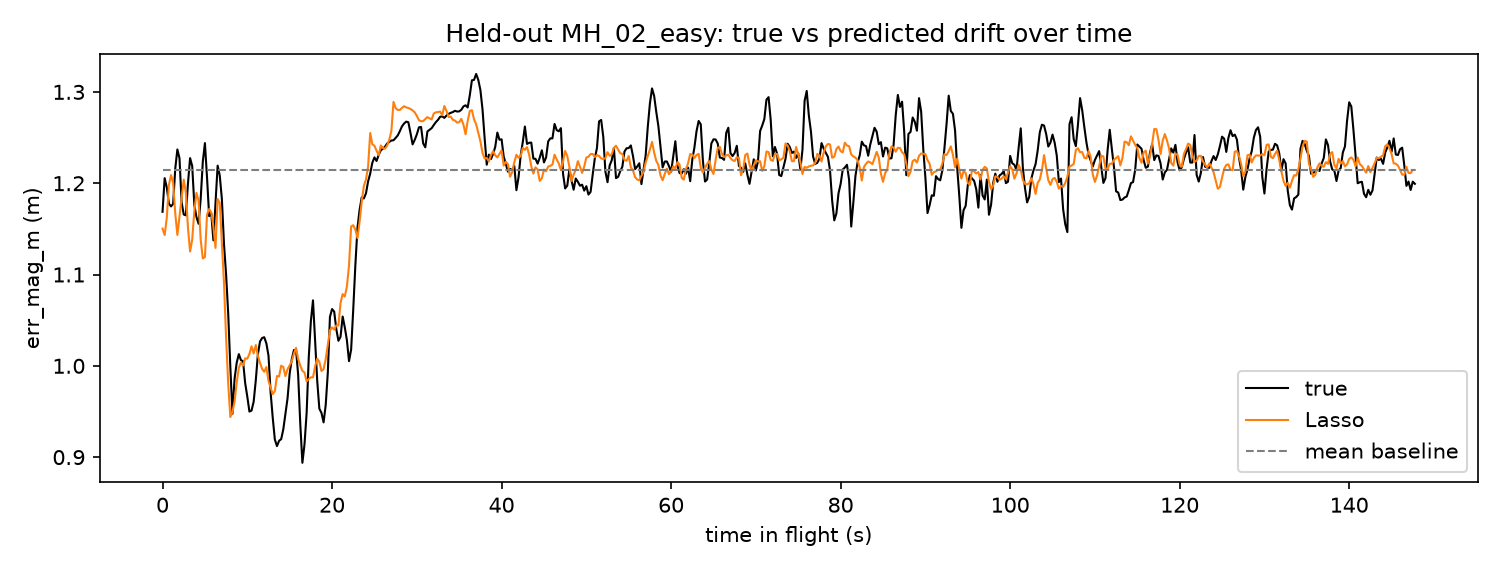
\includegraphics[width=\linewidth]{../../figures/ml/drift_over_time_MH_02_easy.png}
\caption{True drift and Lasso's prediction over the held-out MH\_02\_easy
flight (trained on MH\_01\_easy). Lasso follows the large take-off dip in the
first $\sim$25\,s, but in normal flight its prediction is much smoother than
the truth.}
\label{fig:drift-over-time}
\end{figure}

\subsection{Choosing $\alpha$}
\label{sec:tuning-results}

% Source: results/metrics/err_mag_m.csv (column alpha)
The median rule chose $\alpha = 316$ (trained on MH\_02) and $31.6$ (trained on
MH\_01) for Ridge, and $\alpha = 0.0022$ and $0.00046$ for Lasso.

% Source: results/diagnostics/alpha_sweep_err_mag_m.csv
To check these choices we swept $\alpha$ over the whole grid and scored the
\emph{test} flights (Figure~\ref{fig:alpha-sweep}). This uses test data, so it
is a diagnostic only and played no part in the choice. The curves show the
expected trade-off: at small $\alpha$ the model is essentially OLS, with low
training error but high held-out error; at large $\alpha$ every weight is
pushed to zero and the model becomes the mean baseline. The held-out minimum
lies at $\alpha \approx 100$--$300$ for Ridge and
$\alpha \approx 0.002$--$0.005$ for Lasso on both flights. All four chosen
values fall in the low part of these curves.

\begin{figure}[htbp]
\centering
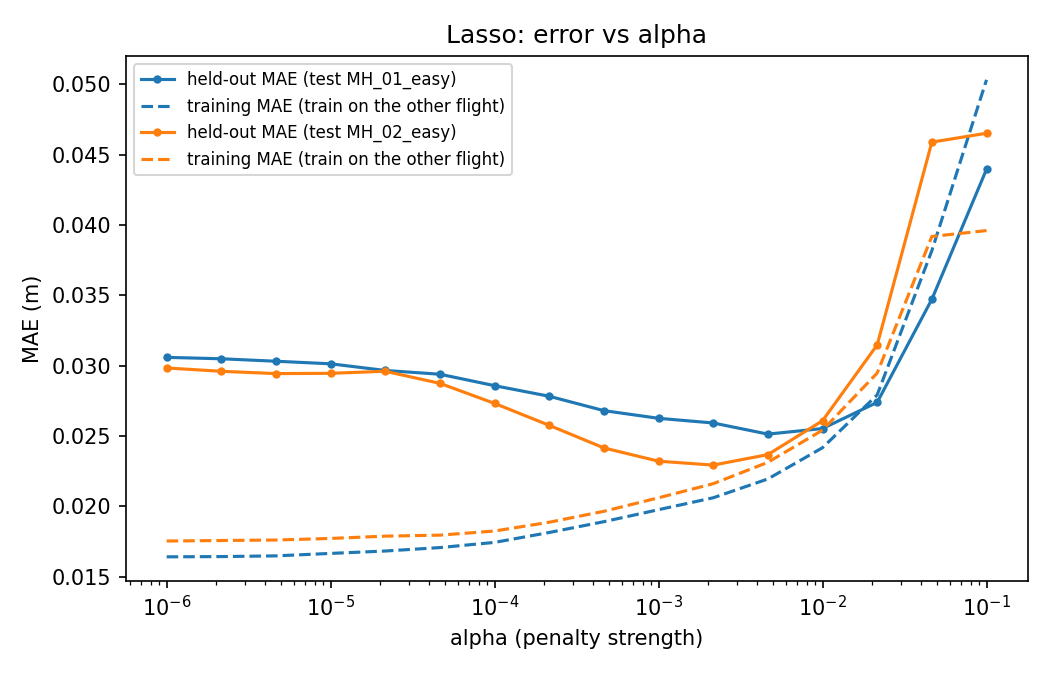
\includegraphics[width=0.8\linewidth]{../../figures/ml/alpha_sweep_lasso.png}
\caption{Lasso training and held-out MAE against $\alpha$, for both folds
(diagnostic only; $\alpha$ is not chosen from this). Ridge shows the same
shape (\texttt{figures/ml/alpha\_sweep\_ridge.png}).}
\label{fig:alpha-sweep}
\end{figure}

% Source: results/diagnostics/tuning_check_err_mag_m.csv (n_blocks = 5)
The median rule matters. With the same 5 blocks, the usual mean rule, trained
on MH\_01, chose Ridge $\alpha = 3.2 \times 10^4$ (held-out $R^2 = 0.32$ instead
of 0.80). The one-standard-error rule was worse: it chose the largest $\alpha$
in the grid for both Ridge ($R^2 = 0.13$) and Lasso, where $\alpha = 0.1$ zeroes
every weight ($R^2 = -0.02$). Trained on MH\_02, all three rules gave good
choices. With 3, 5, 8 or 10 blocks, the median rule never chose an $\alpha$
that zeroes every Lasso weight; with 5 or more blocks it gave Lasso
$R^2 = 0.68$ on MH\_01 and 0.84--0.85 on MH\_02. Tuning on a single flight
remains noisy, though: the median curve itself is bumpy (notebook~05).

\subsection{Over-fitting}
\label{sec:overfitting}

% Source: results/metrics/err_mag_m.csv (columns train_mae, mae, "mean" rows)
\begin{table}[htbp]
\centering
\caption{Training vs.\ held-out MAE, mean of the two folds.}
\label{tab:overfit}
\begin{tabular}{lrrr}
\hline
Model & Train MAE (cm) & Held-out MAE (cm) & Held-out / train \\
\hline
Mean baseline & 4.50 & 4.53 & 1.01 \\
OLS           & 1.65 & 2.99 & 1.81 \\
Ridge (L2)    & 1.95 & 2.70 & 1.38 \\
Lasso (L1)    & 2.01 & 2.50 & 1.24 \\
\hline
\end{tabular}
\end{table}

OLS fits its training flight almost twice as well as the new flight
(Table~\ref{tab:overfit}): with 104 correlated features and about 600 windows
it learns flight-specific noise. The penalties trade a slightly worse training
fit for a clearly better held-out one: the held-out/train ratio falls from 1.81
to 1.38 (Ridge) and 1.24 (Lasso). Lasso does this with few features: it keeps
18 of the 104 when trained on MH\_02 and 40 when trained on MH\_01, and 9 are
kept in both folds, including the accelerometer means and RMS, which encode
the window's tilt against gravity (notebook~05).

\subsection{What the models capture}
\label{sec:segments}

% Source: notebooks/06_model_evaluation.ipynb, Section 5
\begin{table}[htbp]
\centering
\caption{Lasso's held-out $R^2$ and MAE in the first 20\% of each flight
(take-off) and in the remaining 80\%, with the mean baseline's MAE.}
\label{tab:segments}
\begin{tabular}{llrrr}
\hline
Test flight & Part & Lasso $R^2$ & Lasso MAE (cm) & Baseline MAE (cm) \\
\hline
MH\_01 & first 20\% & 0.86 & 2.85 & 8.77 \\
       & remaining 80\% & 0.10 & 2.53 & 3.30 \\
MH\_02 & first 20\% & 0.84 & 3.60 & 13.03 \\
       & remaining 80\% & 0.17 & 2.12 & 2.57 \\
\hline
\end{tabular}
\end{table}

The $R^2$ in Table~\ref{tab:heldout} has to be read with care. Most of a
flight's drift variation is the take-off dip, from about 1.22\,m down to about
1.0\,m (Figure~\ref{fig:drift-over-time}). The models track this slow, large
change well: Lasso reaches $R^2 = 0.84$--$0.86$ in the first 20\% of each
flight (Table~\ref{tab:segments}), and that segment dominates the whole-flight
$R^2$. In normal flight Lasso explains only a small part of the fast
window-to-window changes ($R^2 = 0.10$--$0.17$); its predictions are much
smoother than the truth. It still beats the baseline there in MAE (2.53 vs
3.30\,cm on MH\_01, 2.12 vs 2.57\,cm on MH\_02). Ridge and OLS show the same
pattern ($R^2$ 0.50--0.77 in the first 20\%, $-0.17$ to 0.11 in the rest).

\subsection{Window length}
\label{sec:window-length}

% Source: results/diagnostics/window_length_ceiling.csv (target err_mag_m,
% mean of the two test flights)
\begin{table}[htbp]
\centering
\caption{Mean held-out $R^2$ of \texttt{err\_mag\_m} over the two folds, by
window length, for bias-based predictors.}
\label{tab:window-length}
\begin{tabular}{lrrrr}
\hline
Window length & 0.5\,s & 1\,s & 1.5\,s & 2\,s \\
\hline
Physics feature, no fitting & 0.06 & 0.47 & 0.70 & 0.82 \\
Physics feature, linear fit & 0.13 & 0.48 & 0.70 & 0.82 \\
Oracle ceiling (true bias)  & 0.15 & 0.51 & 0.72 & 0.83 \\
\hline
\end{tabular}
\end{table}

The first version of this pipeline used 1\,s windows. Because the raw label is
mostly integrated bias, whose position error grows quickly with time, while the
rest behaves like noise from window to window, a longer window should make the
label more predictable. To test this without rebuilding the 104 features, every
flight was re-windowed at 0.5--2\,s and scored with three bias-based
predictors (Table~\ref{tab:window-length}): the physics feature
\texttt{phys\_mag} used directly (Section~\ref{sec:physics-feature}); a linear
fit $y \approx a + c \cdot \texttt{phys\_mag}$ on the training flight; and an
\emph{oracle} fit on the test flight's own drift from its true bias, which no
real model can know and which bounds what a bias-based predictor can reach.
All three rise steadily with window length; at 1\,s even the oracle explains
only about half of the variation, against 0.83 at 2\,s. This is why the window
was changed to 2\,s.

The table also shows that the physics feature alone, with no fitting, reaches
$R^2 = 0.82$ at 2\,s, above Lasso's 0.76 on the 104 motion features
(Table~\ref{tab:heldout}). Adding it to the models is the obvious next step.
Like the label, it uses the ground-truth state at the start of each window.

\subsection{Limitations}

With only two flights, every result rests on two folds, and each model is tuned
on a single flight. Both flights are ``easy'' Machine Hall sequences with the
same sensor, so the results say nothing yet about faster or more aggressive
flights. And as Section~\ref{sec:segments} shows, much of the explained
variation comes from the take-off.


\bibliographystyle{plain}
\bibliography{references}

\end{document}
